\chapter{Guided Reading: Selberg's Theorem at Many Points}
\label{ch:selberg}

\begin{center}\itshape
At one random height, $\log|\zeta|$ is a Gaussian.\\
At two heights far apart, two independent Gaussians.\\
At two heights very close together, the same Gaussian twice.\\
In between lies a whole geometry.
\end{center}

Volume~14 ends its Chapter~7 with Selberg's central limit theorem: for $t$ uniform on $[T,2T]$, $\log|\zeta(\frac12+it)|$ divided by $\sqrt{\frac12\log\log T}$ tends to a standard Gaussian. Selberg proved it in 1946 with a method that controls the zeros of $\zeta$ by a density estimate of his own. Seventy years later Maksym Radziwi\l\l{} and Kannan Soundararajan found a short proof that needs almost nothing about the zeros, and that is the proof Volume~14 gives. This chapter reads their paper, and then asks the next question, which the theorem at one point cannot answer: \emph{how do the values of $\zeta$ at nearby points depend on each other?}

The answer was found by Paul Bourgade in 2010, in a paper called \emph{Mesoscopic fluctuations of the zeta zeros}. It is that $\log|\zeta(\frac12+it)|$, viewed as a random function of a shift $h$, is a \emph{log-correlated Gaussian field}: two points at distance $h$ share a fraction
\[
\frac{\log(1/|h|)}{\log\log T}
\]
of their randomness, as long as $\frac1{\log T}\le|h|\le1$. This is the structure of the branching random walk of Chapter~\ref{ch:chaos}, and of the characteristic polynomial of a random unitary matrix (Volume~11, Proposition~12.3). It is the reason why the maximum of $|\zeta|$ on a short interval is now one of the best understood questions about $\zeta$. We prove the theorem, with Volume~14 doing the analytic work.

\section{How to read Radziwi\l\l{} and Soundararajan}

The paper, \emph{Selberg's central limit theorem for $\log|\zeta(\frac12+it)|$} (L'Enseignement Math\'ematique, 2017), is short and every line counts. Before reading the proofs, read the introduction until you can say the four steps out loud.
\begin{enumerate}
\item \emph{Move off the line.} Replace $\frac12$ by $\sigma_0=\frac12+\frac W{\log T}$ with $W=(\log\log\log T)^4$. The cost is controlled by an average over the zeros, with no zero density estimate: Volume~14, Proposition~7.3 and Corollary~7.4.
\item \emph{The prime sum is Gaussian.} At $\sigma_0$, the Dirichlet polynomial $P(s)=\sum_{n\le X}\frac{\Lambda(n)}{n^s\log n}$, with $X=T^{1/(\log\log\log T)^2}$, has Gaussian real part, by the method of moments and the mean value theorem for Dirichlet polynomials: Volume~14, Lemma~7.5 and Proposition~7.7.
\item \emph{Mollify.} A short Dirichlet polynomial $M$ satisfies $Me^P\approx1$ (Volume~14, Proposition~7.11).
\item \emph{Compare with $\zeta$.} A twisted second moment of $\zeta$ (Volume~14, Theorem~7.14) shows $\zeta M\approx1$ in mean square (Proposition~7.16).
\end{enumerate}
The parameters look strange until you see what each one is for. $W$ must be $o(\sqrt{\log\log T})$, so that step 1 costs less than the standard deviation, and $W$ must be large compared with $\frac{\log T}{\log X}$, so that the mollifier of step~3 reaches the primes where the damping $p^{-(2\sigma_0-1)}$ starts to bite. Every power of $\log\log\log T$ in the paper is there to make two such requirements meet. A good exercise on a second reading is to replace $W$ by $(\log\log\log T)^a$ and find the range of $a$ for which the proof still works.

What we need from the paper is the conclusion of its argument, which Volume~14 establishes in the proof of Theorem~7.1 (with Proposition~7.7 for the passage from $P$ to its prime part): writing $L_2=\log\log T$, $P_0(s)=\sum_{p\le X}p^{-s}$, and $u$ uniform on $[T,2T]$,
\begin{equation}\label{eq:rsapprox}
\frac{\log|\zeta(\frac12+iu)|-\operatorname{Re}P_0(\sigma_0+iu)}{\sqrt{L_2}}\longrightarrow0
\end{equation}
in probability. 
Everything about $\zeta$ in this chapter comes from \eqref{eq:rsapprox}; everything else is about primes.

\section{Two points}

Volume~14, Exercise~7.4, shows that for a \emph{fixed} shift $h\ne0$ the prime sums at $t$ and at $t+h$ become independent. The reason is that their covariance is the oscillating sum
\[
C_T(h)=\sum_{p\le X}\frac{\cos(h\log p)}{p^{2\sigma_0}},
\]
which stays bounded, while the variances $C_T(0)=v_T$ grow like $\log\log T$. When $h$ shrinks with $T$, the primes with $\log p\le\frac1{|h|}$ do not oscillate: $\cos(h\log p)\approx1$. So the covariance should be about $\sum_{p\le e^{1/|h|}}\frac1p\approx\log\frac1{|h|}$, as long as this is less than $L_2$. The next lemma makes this precise, uniformly in $h$. Throughout, $W$, $\sigma_0$ and $X$ are the parameters of Volume~14, and $\delta=2\sigma_0-1=\frac{2W}{\log T}$; note $\log W=4\log\log\log\log T=o(L_2)$.

\begin{lemma}[the covariance of the prime sums]\label{lem:covariance}
There is an absolute constant $C$ such that, for $T$ large and every real $h$ with $0<|h|\le1$,
\[
\Bigl|C_T(h)-\min\Bigl(\log\frac1{|h|},L_2\Bigr)\Bigr|\le C\log W .
\]
Also $|C_T(0)-L_2|\le C\log W$.
\end{lemma}

\begin{proof}
The case $h=0$ is Volume~14, Proposition~7.7 ($C_T(0)=v_T$). Let $0<|h|\le1$ and $Z=\min(e^{1/|h|},T^{1/W})$; then $Z\ge e$ and $Z\le X$ for $T$ large (since $W\ge(\log\log\log T)^2$). We use Mertens's estimates (Volume~5): $\sum_{p\le y}\frac1p=\log\log y+M+O(\frac1{\log y})$ and $\sum_{p\le y}\frac{\log p}p\le\log y+C_0$.

\emph{Small primes, $p\le Z$.} Here $|h|\log p\le1$ and $\delta\log p\le\delta\log T^{1/W}=2$. From $\cos x\ge1-\frac{x^2}2$ and $e^{-y}\ge1-y$,
\[
1\ge\cos(h\log p)\,p^{-\delta}\ge1-\frac{h^2\log^2p}2-\delta\log p,
\]
and the sum of the error terms over $p\le Z$, weighted by $\frac1p$, is at most $\frac{h^2}2\log Z\,(\log Z+C_0)+\delta(\log Z+C_0)\le\frac12+C_0+2+C_0$. So $\sum_{p\le Z}\frac{\cos(h\log p)}{p^{1+\delta}}=\log\log Z+O(1)$.

\emph{Large primes, $Z<p\le X$, when $Z=T^{1/W}$.} Bound the terms by $\frac1p$: their sum is at most $\log\frac{\log X}{\log Z}+O(1)=\log\frac W{(\log\log\log T)^2}+O(1)\le\log W+O(1)$. And in this case $\log\log Z=L_2-\log W$ while $\log\frac1{|h|}\ge L_2-\log W$, so $\min(\log\frac1{|h|},L_2)$ lies in $[L_2-\log W,L_2]$. The claim follows.

\emph{Large primes, $Z<p\le X$, when $Z=e^{1/|h|}<T^{1/W}$.} Now $\log\log Z=\log\frac1{|h|}<L_2$, and it remains to show that $S=\sum_{Z<p\le X}p^{-1-\delta-ih}$ is bounded, since the sum we want is its real part. By the prime number theorem with error term (Volume~5, Corollary~7.9), $\pi(u)=\operatorname{li}(u)+R(u)$ with $|R(u)|\le\frac{C_1u}{\log^2u}$ for $u\ge2$, where $\operatorname{li}(u)=\int_2^u\frac{\dd v}{\log v}$. With $f(u)=u^{-1-\delta-ih}$, so that $|f(u)|\le\frac1u$ and $|f'(u)|\le\frac3{u^2}$,
\[
S=\int_Z^X\frac{f(u)}{\log u}\dd u+\Bigl[f(u)R(u)\Bigr]_Z^X-\int_Z^XR(u)f'(u)\dd u .
\]
The last two terms are at most $\frac{2C_1}{\log^2Z}+3C_1\int_Z^\infty\frac{\dd u}{u\log^2u}\le\frac{5C_1}{\log Z}\le5C_1$. In the first, put $u=e^v$ and $z=\delta+ih$; it becomes $\int_a^be^{-zv}\frac{\dd v}v$ with $a=\log Z=\frac1{|h|}$, and one integration by parts gives
\[
\int_a^be^{-zv}\frac{\dd v}v=\Bigl[\frac{e^{-zv}}{-zv}\Bigr]_a^b-\int_a^b\frac{e^{-zv}}{zv^2}\dd v,\qquad\Bigl|\int_a^be^{-zv}\frac{\dd v}v\Bigr|\le\frac2{|z|a}+\frac1{|z|a}\le3,
\]
since $|e^{-zv}|\le1$ and $|z|\ge|h|=\frac1a$. So $|S|\le3+5C_1$.
\end{proof}

The lemma says that the correlation between the two prime sums is
\[
\frac{C_T(h)}{C_T(0)}=\frac{\min(\log\frac1{|h|},\log\log T)}{\log\log T}+o(1):
\]
it is $1$ for $|h|\le\frac1{\log T}$, $0$ for $|h|\ge\frac1{(\log T)^{\varepsilon}}$ whatever $\varepsilon>0$, and $a$ for $|h|=(\log T)^{-a}$. The scale $\frac1{\log T}$ is the mean spacing of the zeros (up to $2\pi$), which is no coincidence: below it, $\zeta$ has no room to change.

\begin{figure}[ht]\centering\fig{ch04-correlation}
\caption{Correlation between $\log|\zeta(\frac12+it)|$ and $\log|\zeta(\frac12+it+ih)|$ for $1000$ random $t\in[10^6,2\cdot10^6]$, against $h$ on a logarithmic scale (orange); the same correlation for the prime sums $\sum_{p\le10^6}\frac{\cos(t\log p)}{\sqrt p}$, computed exactly as $\sum\frac{\cos(h\log p)}p/\sum\frac1p$ (blue); and the limit shape $\min(\log\frac1h,L_2)/L_2$ with $L_2=\log\log(1.5\cdot10^6)=2.65$ (dashed). At this height $\log\log T$ is small and the transition is spread out: the data fall from $0.99$ at $h=10^{-3}$ to $0.58$ at $h=0.11$ and $0.09$ at $h=0.83$, decaying roughly linearly in $\log h$ over the last decade. Beyond $h=1$ both the data and the prime sums are slightly negative ($-0.05$ and $-0.04$ at $h=1.6$), as in Exercise~\ref{ex:negcov}.}
\label{fig:correlation}
\end{figure}

\section{Many points: the theorem}

\begin{theorem}[a multi-point central limit theorem]\label{thm:multipoint}
Let $k\ge1$, and for each $T$ let $h_1,\dots,h_k\in[-\frac12,\frac12]$ be shifts (depending on $T$). Assume that for all $i,j$,
\[
\frac{\min\bigl(\log\frac1{|h_i-h_j|},\,L_2\bigr)}{L_2}\longrightarrow c_{ij}\qquad(T\to\infty),
\]
with the convention $\log\frac10=+\infty$, so that $c_{ii}=1$. Then the matrix $\Gamma=(c_{ij})$ is positive semi-definite, and for $t$ uniform on $[T,2T]$,
\[
\Bigl(\frac{\log|\zeta(\frac12+it+ih_j)|}{\sqrt{\frac12L_2}}\Bigr)_{1\le j\le k}\longrightarrow\mathcal N(0,\Gamma)\quad\text{in law}.
\]
\end{theorem}

The proof has two steps: the same statement for the prime sums $Y_j=\operatorname{Re}P_0(\sigma_0+it+ih_j)$, by moments, and then the transfer to $\zeta$ by \eqref{eq:rsapprox}. The moment computation is the one of Volume~14, Proposition~7.7 and Exercise~7.4, organised so that the shifts are arbitrary; we give it in full, since everything rests on it.

\begin{lemma}[joint moments]\label{lem:jointmoments}
Let $K\ge1$ and $r\mapsto j(r)$ be any map from $\{1,\dots,K\}$ to $\{1,\dots,k\}$. Then
\[
\mathbb E_T\Bigl[\prod_{r=1}^KY_{j(r)}\Bigr]=\sum_{\pi}\prod_{\{a,b\}\in\pi}\tfrac12C_T\bigl(h_{j(a)}-h_{j(b)}\bigr)+O_K\bigl(v_T^{K/2-2}\bigr)+o(1),
\]
where $\pi$ runs over the perfect matchings of $\{1,\dots,K\}$ (partitions into pairs; none if $K$ is odd), and the $O$ and $o$ are uniform in the shifts.
\end{lemma}

\begin{proof}
Write $s_r=\sigma_0+it+ih_{j(r)}$ and $c(u)=\sum_{p\le X}p^{-2\sigma_0-iu}$, so that $C_T(u)=\operatorname{Re}c(u)$ and $c(-u)=\overline{c(u)}$. As a function of $t$, $P_0(s_r)=\sum_{p\le X}a_r(p)p^{-it}$ with $a_r(p)=p^{-\sigma_0-ih_{j(r)}}$, a Dirichlet polynomial, and $Y_{j(r)}=\frac12(P_0(s_r)+\overline{P_0(s_r)})$. Expanding,
\[
\prod_{r=1}^KY_{j(r)}=2^{-K}\sum_{S\subseteq\{1,\dots,K\}}A_S(t)\overline{B_S(t)},\qquad A_S=\prod_{r\in S}P_0(s_r),\quad B_S=\prod_{r\notin S}P_0(s_r),
\]
both Dirichlet polynomials in $t$. The coefficients of $A_S$ and $B_S$ are supported on $n\le X^K$ and have $\sum_n|\text{coefficient}|\le\pi(X)^K$, so Volume~14, Lemma~7.5, gives
\[
\frac1T\int_T^{2T}A_S\overline{B_S}\,\dd t=D_S+O\Bigl(\frac{X^{4K}}T\Bigr),\qquad D_S=\sum_{\substack{(p_r)_{r\in S},\,(q_r)_{r\notin S}\\\prod p_r=\prod q_r}}\ \prod_{r\in S}a_r(p_r)\prod_{r\notin S}\overline{a_r(q_r)},
\]
and $X^{4K}/T=T^{4K/(\log\log\log T)^2-1}\to0$. By unique factorisation, $\prod p_r=\prod q_r$ forces $|S|=K-|S|$, so $D_S=0$ unless $|S|=K/2$.

Let $|S|=K/2$. Call a tuple $(p_r)_{r\in S}$ \emph{distinct} if its primes are pairwise distinct. For a distinct tuple, the tuples $(q_r)_{r\notin S}$ with the same product are its rearrangements, which correspond exactly to the bijections $\varphi:S^c\to S$, via $q_r=p_{\varphi(r)}$. Hence the distinct tuples contribute
\[
\sum_{\varphi}\ \sum_{(p_r)\text{ distinct}}\ \prod_{r\in S}p_r^{-2\sigma_0}p_r^{-i(h_{j(r)}-h_{j(\varphi^{-1}(r))})}.
\]
Dropping the word ``distinct'' turns the inner sum into the product $\prod_{r\in S}c(h_{j(r)}-h_{j(\varphi^{-1}(r))})$; the tuples with a repeated prime have total weight at most
\[
\binom{K/2}2v_T^{K/2-2}\sum_pp^{-4\sigma_0}\le K^2v_T^{K/2-2}
\]
in absolute value. The non-distinct tuples $(p_r)$ also contribute to $D_S$ directly, with at most $(K/2)!$ rearrangements each, so at most $(K/2)!\,K^2v_T^{K/2-2}$ in absolute value. Thus
\[
D_S=\sum_{\varphi:S^c\to S}\ \prod_{r\in S}c\bigl(h_{j(r)}-h_{j(\varphi^{-1}(r))}\bigr)+O_K\bigl(v_T^{K/2-2}\bigr).
\]
Now a pair $(S,\varphi)$ is the same thing as a perfect matching $\pi$ of $\{1,\dots,K\}$, the pairs being $\{r,\varphi^{-1}(r)\}$ for $r\in S$, together with a choice, in each pair, of the element that lies in $S$. The pair $\{a,b\}$ contributes $c(h_{j(a)}-h_{j(b)})$ if $a\in S$ and $c(h_{j(b)}-h_{j(a)})$ if $b\in S$; summing over the two choices in every pair,
\[
\begin{aligned}
2^{-K}\sum_SD_S&=2^{-K}\sum_\pi\prod_{\{a,b\}\in\pi}2\operatorname{Re}c\bigl(h_{j(a)}-h_{j(b)}\bigr)+O_K(v_T^{K/2-2})\\
&=\sum_\pi\prod_{\{a,b\}\in\pi}\tfrac12C_T\bigl(h_{j(a)}-h_{j(b)}\bigr)+O_K(v_T^{K/2-2}).
\end{aligned}
\]
None of the bounds depends on the shifts.
\end{proof}

The right-hand side is \emph{Isserlis's formula}: for a centred Gaussian vector $(G_1,\dots,G_k)$ with covariance $\Sigma$, $\mathbb E\prod_rG_{j(r)}=\sum_\pi\prod_{\{a,b\}\in\pi}\Sigma_{j(a)j(b)}$. We will not need the formula itself, only its one-dimensional case, which is the familiar $\mathbb EG^K=(K-1)!!\,\sigma^K$.

\begin{proof}[Proof of Theorem~\ref{thm:multipoint}]
\emph{Prime sums.} Let $\Gamma_T$ be the matrix with entries $C_T(h_i-h_j)/L_2$. Since $|h_i-h_j|\le1$, Lemma~\ref{lem:covariance} gives $\Gamma_T\to\Gamma$ (when $h_i=h_j$ the entry is $C_T(0)/L_2\to1=c_{ij}$). Fix $a\in\R^k$ and put $Z_T=\sum_ja_jY_j/\sqrt{L_2/2}$. Expanding $Z_T^K$ multilinearly and applying Lemma~\ref{lem:jointmoments} to each term,
\[
\mathbb E_T[Z_T^K]=\Bigl(\frac2{L_2}\Bigr)^{K/2}\sum_{j(1),\dots,j(K)}\prod_ra_{j(r)}\Bigl(\sum_\pi\prod_{\{a',b'\}\in\pi}\tfrac12C_T(h_{j(a')}-h_{j(b')})\Bigr)+o(1).
\]
For each matching $\pi$, the sum over $j(1),\dots,j(K)$ factorises over the pairs of $\pi$, each pair giving $\sum_{i,j}a_ia_j\frac12C_T(h_i-h_j)=\frac{L_2}2\,a^{\mathsf T}\Gamma_Ta$. There are $(K-1)!!$ matchings when $K$ is even, so
\[
\mathbb E_T[Z_T^K]=\begin{cases}(K-1)!!\,(a^{\mathsf T}\Gamma_Ta)^{K/2}+o(1),&K\text{ even},\\o(1),&K\text{ odd}.\end{cases}
\]
For $K=2$ this shows $a^{\mathsf T}\Gamma_Ta+o(1)=\mathbb E_TZ_T^2\ge0$, so $a^{\mathsf T}\Gamma a\ge0$ for every $a$: $\Gamma$ is positive semi-definite. If $a^{\mathsf T}\Gamma a=0$, then $\mathbb E_TZ_T^2\to0$ and $Z_T\to0=\mathcal N(0,a^{\mathsf T}\Gamma a)$. Otherwise the moments of $Z_T/\sqrt{a^{\mathsf T}\Gamma a}$ tend to those of a standard Gaussian, and Volume~5, Lemma~9.6, gives $Z_T\to\mathcal N(0,a^{\mathsf T}\Gamma a)$. This is the law of $\sum_ja_jG_j$ for $G\sim\mathcal N(0,\Gamma)$, so by the Cram\'er--Wold device (Volume~10, Corollary~3.4), $(Y_j/\sqrt{L_2/2})_j\to\mathcal N(0,\Gamma)$.

\emph{Transfer to $\zeta$.} Let $\Delta(u)$ be the quotient in \eqref{eq:rsapprox}. For fixed $j$ and $\varepsilon>0$, $u=t+h_j$ is uniform on $[T+h_j,2T+h_j]$, an interval that differs from $[T,2T]$ by a set of measure at most $2|h_j|\le1$. So
\[
P_T\bigl(|\Delta(t+h_j)|>\varepsilon\bigr)\le P\bigl(|\Delta(u)|>\varepsilon\bigr)+\frac1T\longrightarrow0,
\]
with $u$ uniform on $[T,2T]$. Hence the vector $\bigl(\Delta(t+h_j)\bigr)_j$ tends to $0$ in probability, and since $\sqrt{L_2}/\sqrt{L_2/2}=\sqrt2$, the vector of the theorem differs from $(Y_j/\sqrt{L_2/2})_j$ by $\sqrt2(\Delta(t+h_j))_j\to0$. Slutsky's lemma in $\R^k$ (apply the one-dimensional lemma to each linear combination, and Cram\'er--Wold again) finishes the proof.
\end{proof}

\begin{example}[the three regimes]\label{exa:regimes}
Take $k=2$, $h_1=0$, $h_2=h$. If $|h|\le\frac1{\log T}$ then $c_{12}=1$: the two values are asymptotically equal, at the scale $\sqrt{L_2}$. If $|h|=(\log T)^{-a}$ with $0<a<1$, then $c_{12}=a$. If $(\log T)^{-\varepsilon_T}\le|h|\le\frac12$ with $\varepsilon_T\to0$, for instance $h$ fixed or $h=\frac1{\log\log T}$, then $c_{12}=0$: asymptotically independent.
\end{example}

\section{The geometry of the field}

\begin{figure}[ht]\centering
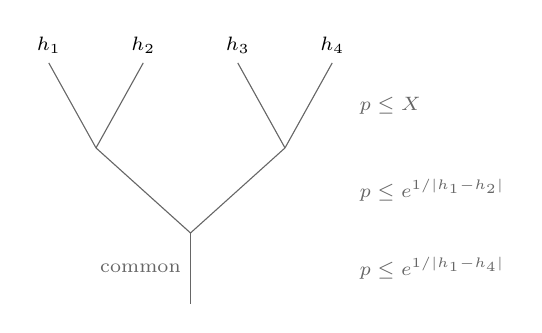
\begin{tikzpicture}[x=0.75cm,y=0.9cm,font=\scriptsize]
\draw[black!60] (0,0)--(0,1) node[midway,left]{common};
\draw[black!60] (0,1)--(-1.6,2.2) (0,1)--(1.6,2.2);
\draw[black!60] (-1.6,2.2)--(-2.4,3.4) (-1.6,2.2)--(-0.8,3.4) (1.6,2.2)--(0.8,3.4) (1.6,2.2)--(2.4,3.4);
\foreach \x/\l in {-2.4/{$h_1$},-0.8/{$h_2$},0.8/{$h_3$},2.4/{$h_4$}} \node[above] at (\x,3.4) {\l};
\node[right,black!60] at (2.7,0.5) {$p\le e^{1/|h_1-h_4|}$};
\node[right,black!60] at (2.7,1.6) {$p\le e^{1/|h_1-h_2|}$};
\node[right,black!60] at (2.7,2.8) {$p\le X$};
\end{tikzpicture}
\caption{Why the field is a tree. The prime sums at $h_i$ and $h_j$ share the primes $p\le e^{1/|h_i-h_j|}$, where $\cos((t+h)\log p)$ barely depends on $h$, and see independent-looking contributions above. Four shifts with $|h_1-h_2|,|h_3-h_4|\ll|h_1-h_3|$ share a common trunk and then split in pairs: the branching random walk of Chapter~\ref{ch:chaos}, with generation $n$ corresponding to the primes $p\approx e^{e^n}$.}
\label{fig:fieldtree}
\end{figure}

For $|h|$ between $\frac1{\log T}$ and $1$, Theorem~\ref{thm:multipoint} gives the covariance $\frac12\log\frac1{|h|}$ for the unnormalised values: in the variable $x=t/\log T$, the values of $\log|\zeta|$ form a Gaussian field with covariance $\frac12\log\frac1{|x-x'|}$ up to the cut-off. This is what probabilists call a \emph{log-correlated field}, and it has the same structure as the field $\log|\det(I-e^{-i\theta}U)|$ of a Haar unitary matrix $U$ of size $N\approx\log\frac T{2\pi}$ (Volume~11, Proposition~12.3). Figure~\ref{fig:fieldtree} explains the tree: grouping the primes by generations $e^{e^{n-1}}<p\le e^{e^n}$, each generation contributes a variance of about $\frac12$, and two shifts at distance $e^{-m}$ share the first $m$ generations exactly.

\begin{remark}[Bourgade's theorem]\label{rem:bourgade}
Bourgade's paper proves more than Theorem~\ref{thm:multipoint}: the joint law of the real \emph{and imaginary} parts of $\log\zeta$, hence also of the numbers of zeros in mesoscopic intervals, whose fluctuations are the increments of $\frac1\pi\operatorname{Im}\log\zeta$. The imaginary part needs a separate argument, for the reason given in Volume~14, Chapter~7 (the mollifier sees $|\zeta|$ but not its argument).
\end{remark}

\begin{remark}[the maximum on a short interval]\label{rem:fhk}
The log-correlated structure governs extremes. Volume~11, Chapter~12, tells the story of the conjecture made in 2012 by Fyodorov, Hiary and Keating, from the random matrix analogy and numerical evidence, and proves the upper bound for the random matrix maximum (Theorem~12.6; the sharp result is Theorem~12.7, admitted there). The conjecture says that for $t$ uniform on $[T,2T]$,
\[
\max_{|h|\le1}\log|\zeta(\tfrac12+it+ih)|=\log\log T-\tfrac34\log\log\log T+O_P(1),
\]
which is exactly the maximum of a branching random walk with $\log\log T$ generations and the variance and branching of Figure~\ref{fig:fieldtree}: the $-\frac34$ is the same ballot correction as in the barrier argument of Chapter~\ref{ch:chaos}. The leading term was proved by Najnudel (2018, under the Riemann hypothesis) and by Arguin, Belius, Bourgade, Radziwi\l\l{} and Soundararajan (2019, unconditionally), and the full conjecture, with the $-\frac34$, by Arguin, Bourgade and Radziwi\l\l{} in two papers (2020 and 2023).
\end{remark}

\begin{beauty}
The primes up to $T$ make $\log|\zeta(\frac12+it)|$, a single Gaussian of variance $\frac12\log\log T$. Move $t$ a little, by $(\log T)^{-a}$, and only the primes beyond $e^{(\log T)^a}$ notice: they are the leaves of a tree whose trunk is the small primes. The zeta function, which has nothing random in it, carries on its critical line the same random tree as a branching population and a random matrix. Each prime is one generation's worth of branching.
\end{beauty}

\section{Exercises}

\begin{exercise}[$\star$]\label{ex:equicorr}
Let $h_j=j(\log T)^{-a}$ for $j=1,\dots,k$, with $0<a<1$. Find $\Gamma$, and check directly that it is positive semi-definite by finding its eigenvalues.
\end{exercise}

\begin{exercise}[$\star\star$]\label{ex:ultrametric}
Let $0<a<b<1$ and $h_1=0$, $h_2=(\log T)^{-b}$, $h_3=(\log T)^{-a}$, $h_4=(\log T)^{-a}+(\log T)^{-b}$. Compute $\Gamma$. Show that in any limit matrix of Theorem~\ref{thm:multipoint}, $c_{ik}\ge\min(c_{ij},c_{jk})$ for all $i,j,k$ (the covariance is \emph{ultrametric}, as for a tree).
\end{exercise}

\begin{exercise}[$\star$]\label{ex:closepoints}
Show that if $|h|\le\frac1{\log T}$, then $\bigl(\log|\zeta(\frac12+it)|-\log|\zeta(\frac12+it+ih)|\bigr)/\sqrt{L_2}\to0$ in probability. Is the same true for $|h|\le\frac{\log\log T}{\log T}$?
\end{exercise}

\begin{exercise}[$\star\star$]\label{ex:increment}
Let $|h|=(\log T)^{-a}$ with $0<a<1$. Find the limit law of $\bigl(\log|\zeta(\frac12+it+ih)|-\log|\zeta(\frac12+it)|\bigr)/\sqrt{L_2}$.
\end{exercise}

\begin{exercise}[$\star\star$]\label{ex:negcov}
Show that $C_T(h)\ge-C\log W$ for $0<|h|\le1$, but that the conclusion of Lemma~\ref{lem:covariance} fails for large $|h|$ in the following sense: $\liminf_{T}\min_{1\le|h|\le2}C_T(h)>-\infty$, while the right-hand side $\min(\log\frac1{|h|},L_2)$ is negative there. Why does Theorem~\ref{thm:multipoint} take its shifts in $[-\frac12,\frac12]$?
\end{exercise}

\begin{exercise}[$\star$]\label{ex:smoothing}
Let $0<a<1$ and $h_j=\frac jk(\log T)^{-a}$ for $j=1,\dots,k$. Find the limit law of $\frac1k\sum_{j\le k}\log|\zeta(\frac12+it+ih_j)|/\sqrt{\frac12L_2}$. How much does averaging over a window of length $(\log T)^{-a}$ reduce the variance, however many points one takes?
\end{exercise}

\section{Hints}

\begin{hint}{ex:equicorr}
All the differences $h_i-h_j$, $i\ne j$, are $(\log T)^{-a}$ times an integer of size at most $k$.
\end{hint}

\begin{hint}{ex:ultrametric}
Show that
\[
\log\frac1{|h_i-h_k|}\ge\min\Bigl(\log\frac1{|h_i-h_j|},\log\frac1{|h_j-h_k|}\Bigr)-\log2.
\]
\end{hint}

\begin{hint}{ex:closepoints}
Use Theorem~\ref{thm:multipoint} with $k=2$, and compute the variance of the difference of the components of $\mathcal N(0,\Gamma)$.
\end{hint}

\begin{hint}{ex:increment}
A linear image of a Gaussian vector is Gaussian.
\end{hint}

\begin{hint}{ex:negcov}
For the lower bound, look again at the three cases of the proof of Lemma~\ref{lem:covariance}. For $1\le|h|\le2$, the small primes with $|h|\log p\le1$ are only $p\le e$.
\end{hint}

\begin{hint}{ex:smoothing}
Compute $\Gamma$ as in Exercise~\ref{ex:equicorr}, then the variance of the mean of a $\mathcal N(0,\Gamma)$ vector.
\end{hint}

\section{Solutions}

\begin{solution}{ex:equicorr}
\idea Every pair is at the same scale.
\writeup For $i\ne j$, $\log\frac1{|h_i-h_j|}=aL_2-\log|i-j|$, so $c_{ij}=a$; and $c_{ii}=1$. So $\Gamma=(1-a)I+aJ$, with $J$ the all-ones matrix. Its eigenvalues are $1-a$ (on the vectors with sum $0$, multiplicity $k-1$) and $1+(k-1)a$ (on $(1,\dots,1)$), all positive. The limit is $G_j=\sqrt aG_0+\sqrt{1-a}\,G_j'$ with independent standard $G_0,G_j'$: a common part of variance $a$, the primes up to $e^{(\log T)^a}$, and independent parts.
\end{solution}

\begin{solution}{ex:ultrametric}
\idea Distances combine by a maximum, at the logarithmic scale.
\writeup Here $|h_1-h_2|=|h_3-h_4|=(\log T)^{-b}$, and the four other differences are $(\log T)^{-a}(1+o(1))$. So $c_{12}=c_{34}=b$, the other off-diagonal entries are $a$, and the diagonal is $1$: a tree with a trunk of length $a$, two branches splitting further at $b$. For the inequality, $|h_i-h_k|\le|h_i-h_j|+|h_j-h_k|\le2\max(|h_i-h_j|,|h_j-h_k|)$, so $\log\frac1{|h_i-h_k|}\ge\min(\log\frac1{|h_i-h_j|},\log\frac1{|h_j-h_k|})-\log2$. Taking $\min(\cdot,L_2)$, dividing by $L_2$ and letting $T\to\infty$ gives $c_{ik}\ge\min(c_{ij},c_{jk})$.
\end{solution}

\begin{solution}{ex:closepoints}
\idea Two components with correlation $1$ are equal.
\writeup With $h_1=0$, $h_2=h$, $|h|\le\frac1{\log T}$: $\log\frac1{|h|}\ge\log\log T=L_2$, so $c_{12}=1$ and $\Gamma=\begin{psmallmatrix}1&1\\1&1\end{psmallmatrix}$. If $(G_1,G_2)\sim\mathcal N(0,\Gamma)$, then $\operatorname{Var}(G_1-G_2)=1-2+1=0$, so $G_1=G_2$. The difference of the components of the vector of the theorem tends in law to $G_1-G_2=0$, hence in probability to $0$, and multiplying by $\frac1{\sqrt2}$ gives the claim. For $|h|\le\frac{\log\log T}{\log T}$: $\log\frac1{|h|}\ge L_2-\log L_2$, so again $c_{12}=1$, and the answer is yes. Only at distances $(\log T)^{-a}$ with $a<1$ does the correlation drop below $1$.
\end{solution}

\begin{solution}{ex:increment}
\idea The increment is the part of the randomness that the two points do not share.
\writeup Here $c_{12}=a$, and the difference $G_2-G_1$ of a $\mathcal N(0,\Gamma)$ vector is Gaussian with variance $1-2a+1=2(1-a)$. The vector of the theorem uses the normalisation $\sqrt{L_2/2}$, so the difference divided by $\sqrt{L_2}$ tends to $\frac1{\sqrt2}(G_2-G_1)\sim\mathcal N(0,1-a)$. The increment comes from the primes beyond $e^{(\log T)^a}$, whose share of the variance is $1-a$.
\end{solution}

\begin{solution}{ex:negcov}
\idea For $|h|\le1$ the formula is a lower bound in disguise; for $|h|>1$ the small primes are absent.
\writeup For $0<|h|\le1$, Lemma~\ref{lem:covariance} gives $C_T(h)\ge\min(\log\frac1{|h|},L_2)-C\log W\ge-C\log W$, since $\log\frac1{|h|}\ge0$. For $1\le|h|\le2$, run the proof of the third case with $Z=2$ in place of $e^{1/|h|}$: the sum over $2<p\le X$ is $\operatorname{Re}\int_{\log2}^{\log X}e^{-zv}\frac{\dd v}v+O(1)$, bounded by $\frac3{|h|\log2}+O(1)$, so $C_T(h)$ is bounded below uniformly, while $\min(\log\frac1{|h|},L_2)=\log\frac1{|h|}\in[-\log2,0]$. So for $1\le|h|\le2$ both sides are bounded, and the lemma remains true there in the form $C_T(h)=O(1)+O(\log W)$; but for $|h|\to\infty$ the right side $\log\frac1{|h|}\to-\infty$ while $C_T(h)$ stays bounded. This is why the theorem takes $h_j\in[-\frac12,\frac12]$: then $|h_i-h_j|\le1$ and Lemma~\ref{lem:covariance} applies. With the variant above it extends to shifts in $[-1,1]$, with $c_{ij}=0$ when $|h_i-h_j|\ge1$.
\end{solution}

\begin{solution}{ex:smoothing}
\idea Averaging kills only the part of the randomness that the points do not share.
\writeup For $i\ne j$, $|h_i-h_j|=\frac{|i-j|}k(\log T)^{-a}$, so $\log\frac1{|h_i-h_j|}=aL_2+O_k(1)$ and $c_{ij}=a$: $\Gamma=(1-a)I+aJ$. By Theorem~\ref{thm:multipoint} and the continuous mapping theorem, the mean tends to $\frac1k\sum_jG_j$, a centred Gaussian with variance $\frac1{k^2}\mathbf 1^{\mathsf T}\Gamma\mathbf 1=\frac{k(1-a)+k^2a}{k^2}=a+\frac{1-a}k$. So the limit is $\mathcal N(0,a+\frac{1-a}k)$. However large $k$, the variance stays above $a$: the primes up to $e^{(\log T)^a}$ are common to the whole window, and no averaging inside it can remove them. Only the primes beyond, the fraction $1-a$ of the variance, average out.
\end{solution}

\section{Sources}

\begin{itemize}
\item A.~Selberg, Contributions to the theory of the Riemann zeta-function, \emph{Arch.\ Math.\ Naturvid.} 48 (1946), 89--155.
\item M.~Radziwi\l\l, K.~Soundararajan, Selberg's central limit theorem for $\log|\zeta(1/2+it)|$, \emph{Enseign.\ Math.} 63 (2017), 1--19. The paper of the first section; its proof is Volume~14, Chapter~7.
\item P.~Bourgade, Mesoscopic fluctuations of the zeta zeros, \emph{Probab.\ Theory Related Fields} 148 (2010). The multi-point theorem, with the imaginary parts.
\item Y.~V.~Fyodorov, G.~A.~Hiary, J.~P.~Keating, Freezing transition, characteristic polynomials of random matrices, and the Riemann zeta function, \emph{Phys.\ Rev.\ Lett.} 108 (2012), 170601.
\item J.~Najnudel, On the extreme values of the Riemann zeta function on random intervals of the critical line, \emph{Probab.\ Theory Related Fields} 172 (2018).
\item L.-P.~Arguin, D.~Belius, P.~Bourgade, M.~Radziwi\l\l, K.~Soundararajan, Maximum of the Riemann zeta function on a short interval of the critical line, \emph{Comm.\ Pure Appl.\ Math.} 72 (2019).
\item L.-P.~Arguin, P.~Bourgade, M.~Radziwi\l\l, The Fyodorov--Hiary--Keating conjecture, I (2020) and II (2023), arXiv preprints.
\end{itemize}
